\chapter{MCU PCB design} \label{app:mcu}

In this appendix, the design of the MCU PCB is described. This stage serves the purpose of sampling the conditioned radar signals as well as performing the digital data processing (DSP) and wireless transmission of the data.

\section{Features}

The MCU PCB has been designed featuring the needs for interoperation with the other radar node parts. The MCU PCB has the following features:
\begin{itemize}
	\item Integration of the STM32WB15CC \cite{STMicroelectronics2022} MCU
	\item Stable, low-dropout and low-current power delivery to the MCU with low dropout (LDO) voltage regulators
	\item Integrated BLE chip antenna
	\item Two SMA connectors for the input intermediate frequency signals
	\item A micro USB connector for power delivery via a wall plug, mobile device or external battery
	\item Arduino-compatible header pins connected to all pins of the MCU for debugging and testing capabilities
	\item Standard JTAG \cite{JTAG} port for MCU programming and debugging
	\item 4-layer design with dedicated ground and power planes
\end{itemize}

\section{Schematic}
The design is materialised with the corresponding components and connectors in a schematic sheet. The schematic for this circuit is shown in \cref{fig:sch_mcu}.

\begin{figure}[h]
	\centering
	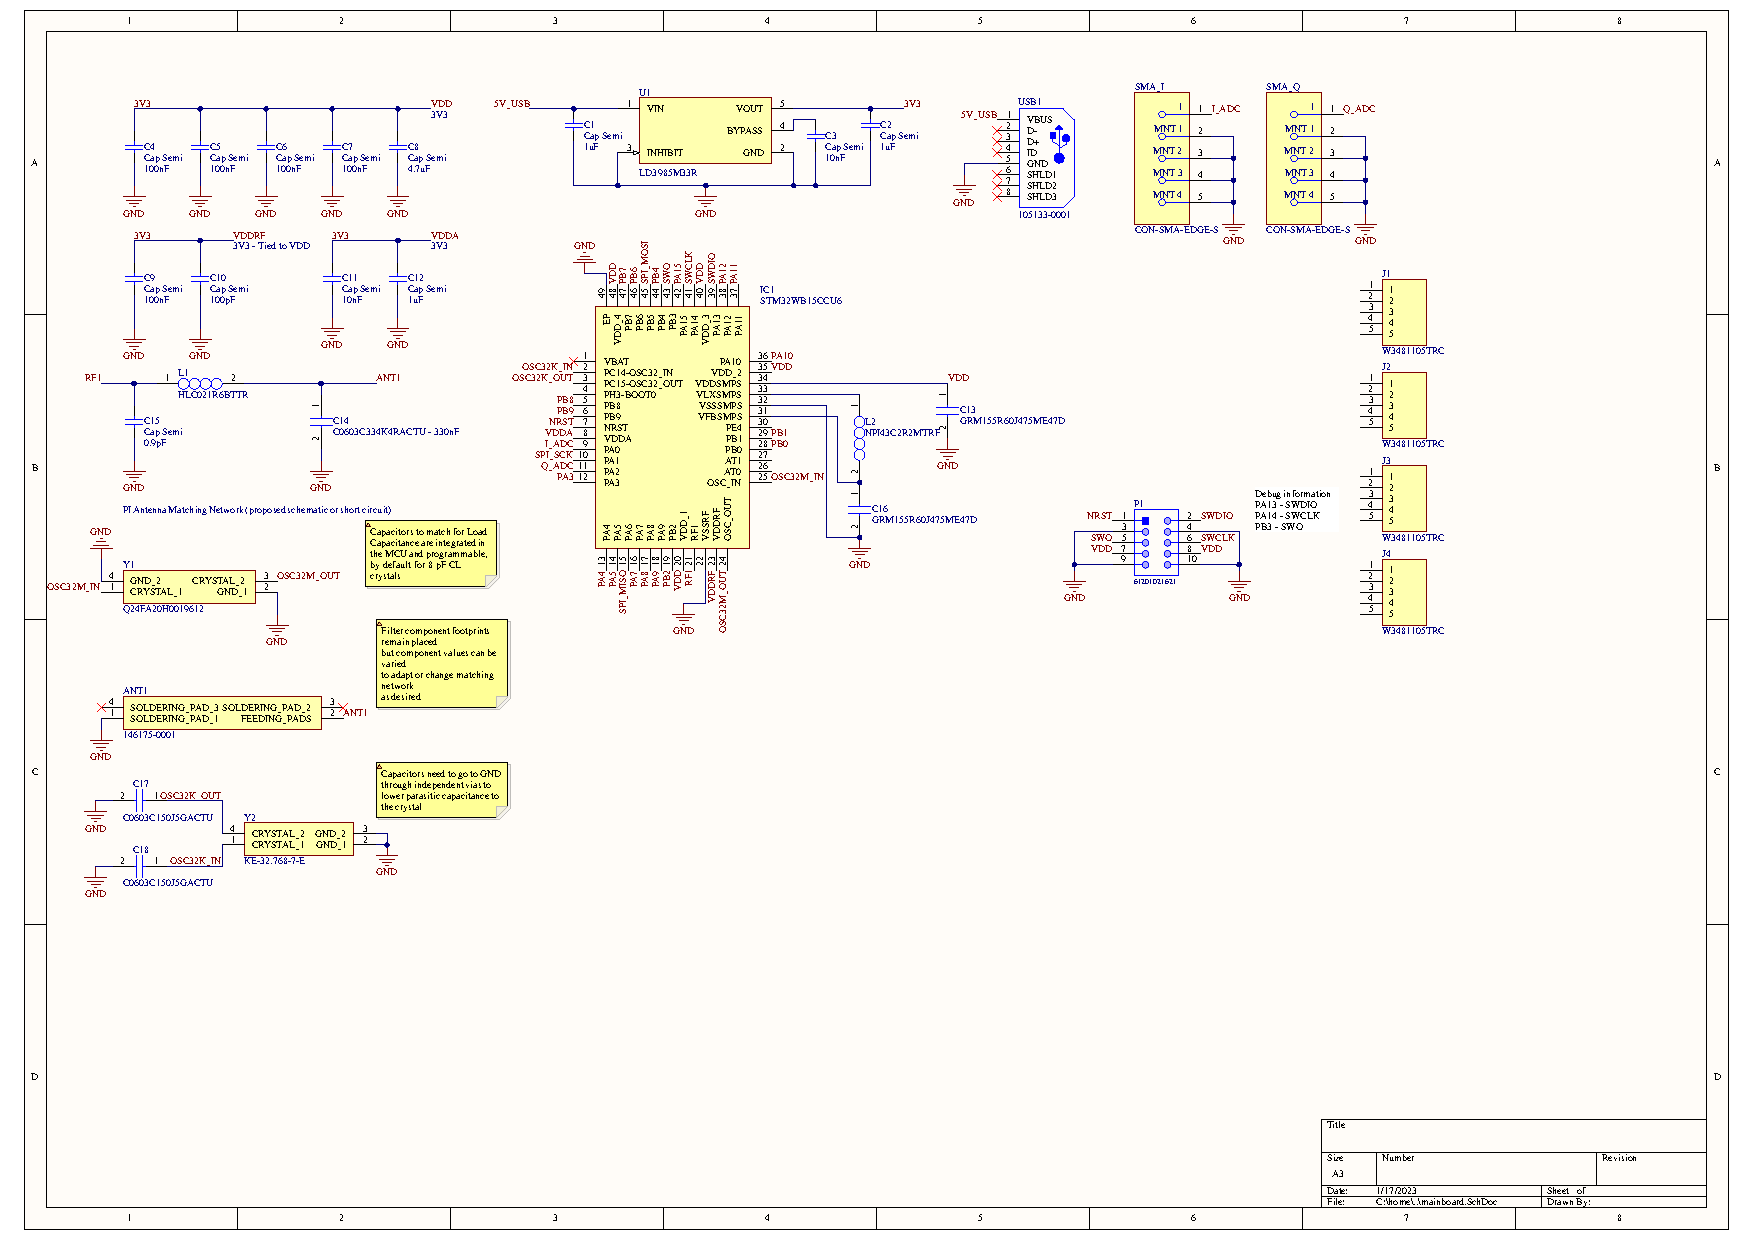
\includegraphics[width=18cm, angle=90]{sch/mcu.pdf}
	\caption{Schematic of the MCU PCB. The MCU is the central piece of the design. The design features a power regulator for MCU power, one connector for USB 5 V power, two SMA connectors for the I and Q conditioned signals, a JTAG programming header and access pins. A BLE antenna is also connected through a RF trace with a matching network in PI configuration. The values of the elements on the matching network are placeholders, the antenna is measured when fabricated and is matched accordingly.}
	\label{fig:sch_mcu}
\end{figure}

\section{Layout}
The schematic components and nets are laid out in a PCB layout. The corresponding connecting nets and components are routed and the PCB layout is designed. The layout for this PCB is shown in \cref{fig:lay_mcu}. Some 3D renders of the PCB are shown in \cref{fig:lay_mcu_3d}.

\begin{figure}[h]
	\centering
	\subfloat[Top layers (signal and overlay).]{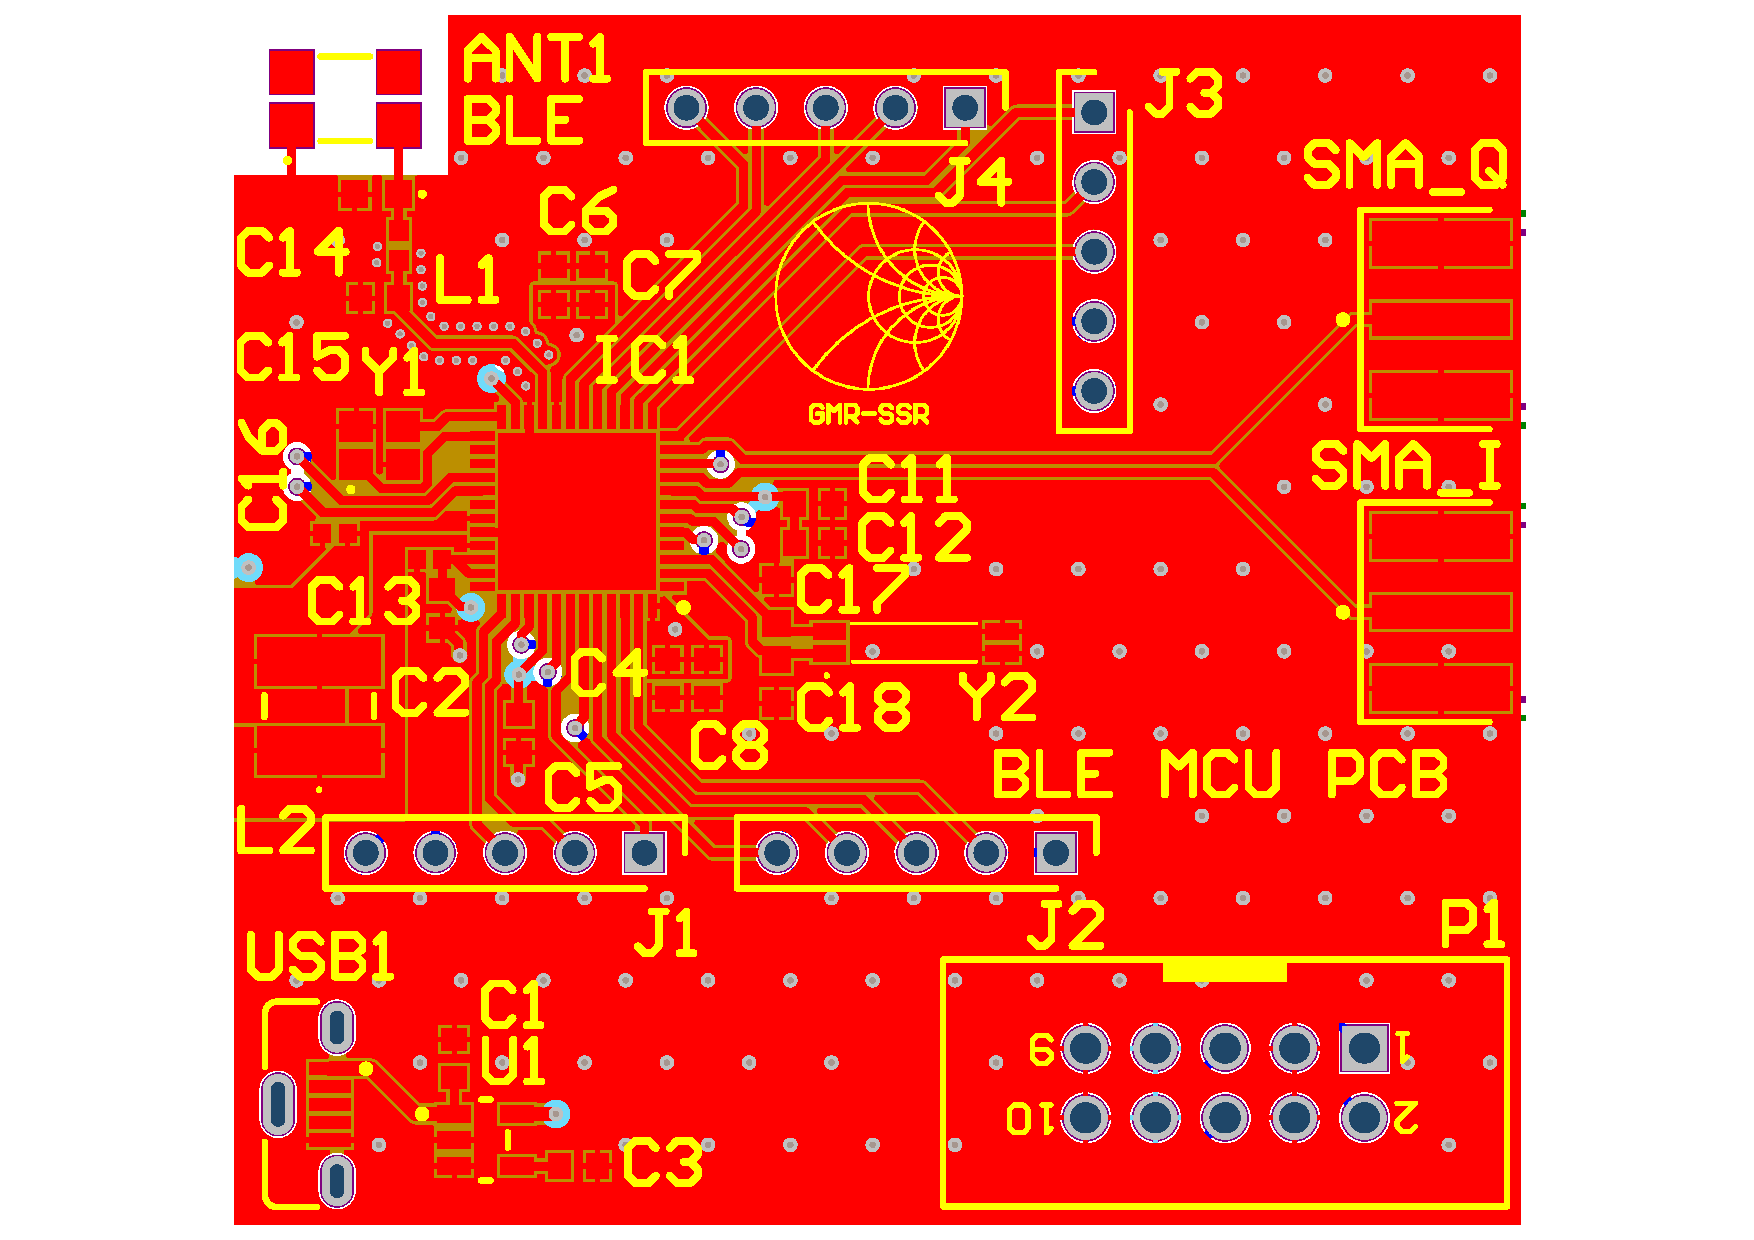
\includegraphics[width=\textwidth, page=1]{lay/pcb_mcu.pdf}}\\
	\subfloat[Bottom layers (signal and overlay).]{\includegraphics[width=\textwidth, page=2]{lay/pcb_mcu.pdf}}
	\caption{Layout of the MCU PCB in different views. The bottom view is mirrored. Vias are represented as grey holes.}
	\label{fig:lay_mcu}
\end{figure}

\begin{figure}[h]
	\centering
	\subfloat[From the top side.]{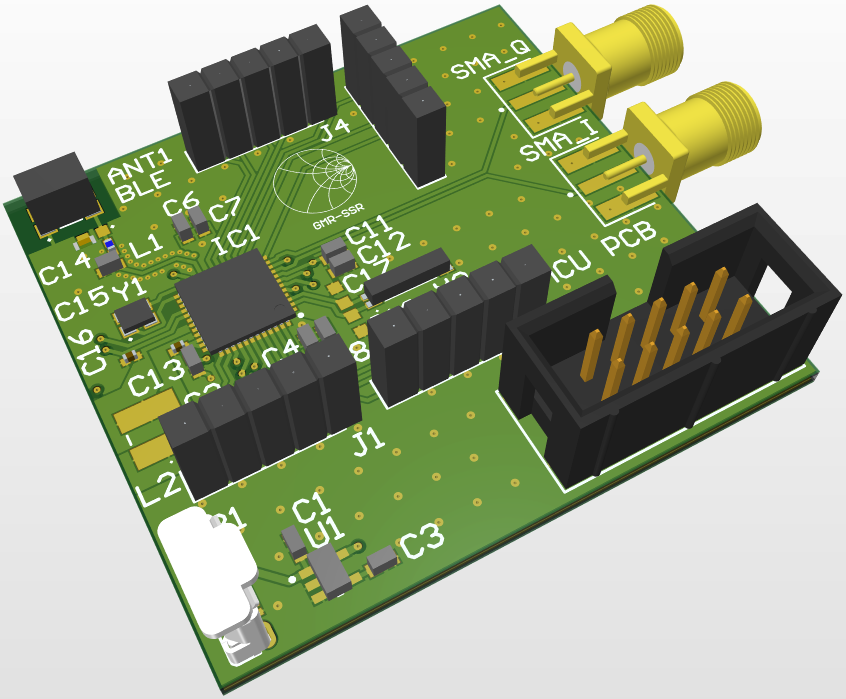
\includegraphics[width=0.7\textwidth]{3d/pcb_mcu_1}}\\
	\subfloat[From the bottom side.]{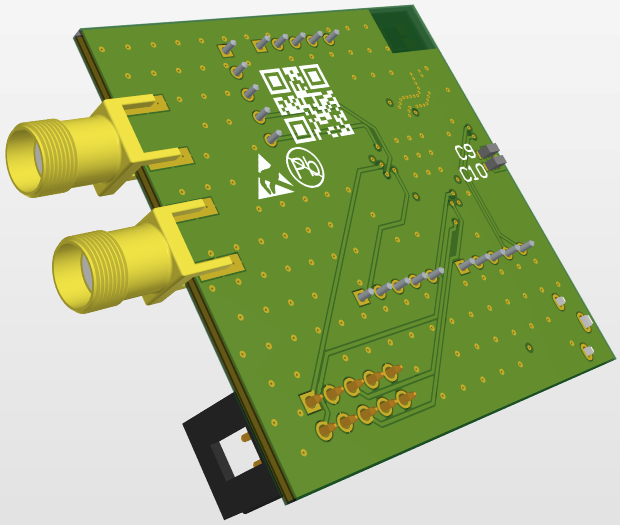
\includegraphics[width=0.7\textwidth]{3d/pcb_mcu_2}}
	\caption{3D renders of the MCU PCB.}
	\label{fig:lay_mcu_3d}
\end{figure}
